% Requires \usepackage{graphicx}. Paths assume thesis/ is next to the .tex file.
% See figures/CAPTIONS.md for full methodological captions.

\begin{figure}[t]
  \centering
  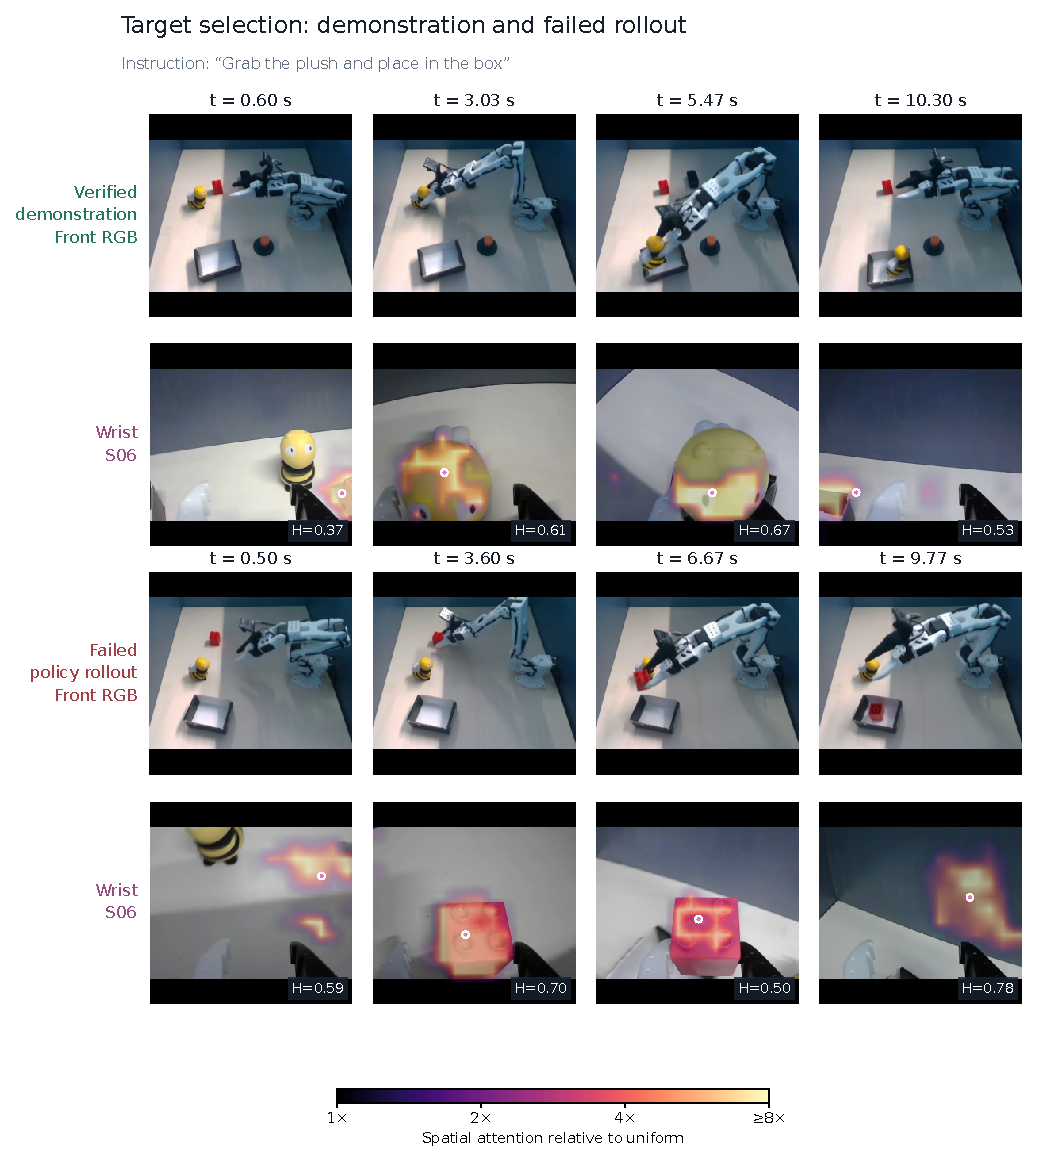
\includegraphics[width=\linewidth]{thesis/figures/main/M01_target_selection.pdf}
  \caption{Recorded target-selection contrast for the instruction ``Grab the plush and place in the box. Front RGB and spatial attention of the same wrist query S06 are shown for a verified demonstration and a failed policy rollout. Frames are selected at the displayed times; scene configurations are not controlled. Heatmap scales are shared.}
  \label{fig:afa-m01}
\end{figure}

\begin{figure}[t]
  \centering
  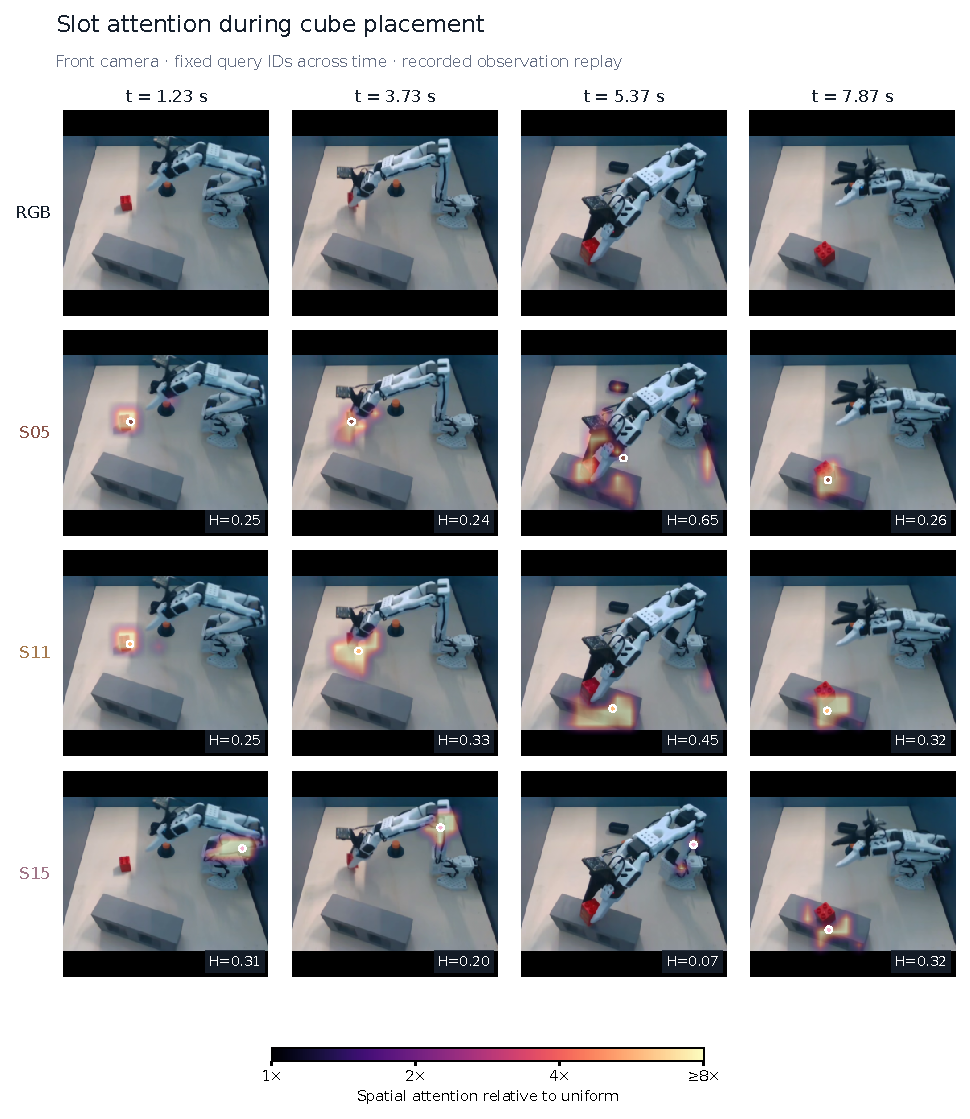
\includegraphics[width=\linewidth]{thesis/figures/main/M02_cube_slot_evolution.pdf}
  \caption{Spatial attention of fixed queries S05, S11 and S15 during a verified cube-placement demonstration. Columns show selected stages of the recorded interaction. Query IDs remain fixed, without instance matching. H is normalized spatial entropy; all heatmaps use the same attention-to-uniform scale.}
  \label{fig:afa-m02}
\end{figure}

\begin{figure}[t]
  \centering
  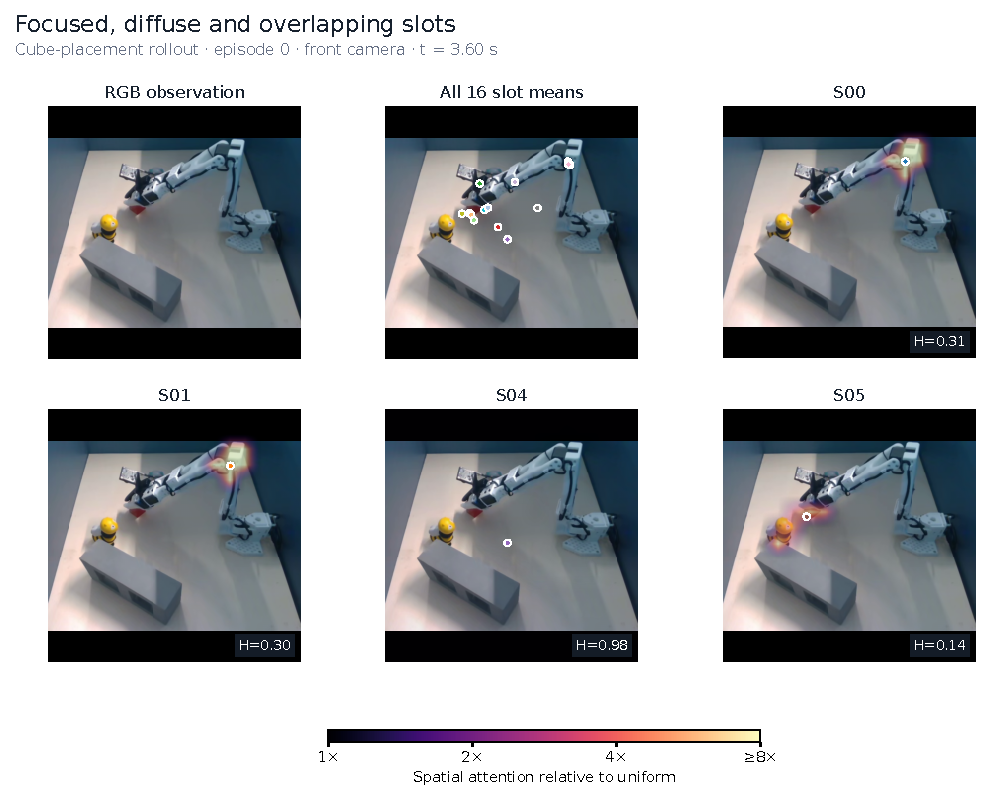
\includegraphics[width=\linewidth]{thesis/figures/main/M03_pooling_diversity.pdf}
  \caption{Concentrated, diffuse and overlapping AFA pooling in one recorded observation. S00 and S01 have similar spatial maps, S04 is diffuse and S05 is more concentrated. All 16 slot means are shown for context. Selected query IDs do not denote annotated object categories.}
  \label{fig:afa-m03}
\end{figure}
